% Options for packages loaded elsewhere
\PassOptionsToPackage{unicode}{hyperref}
\PassOptionsToPackage{hyphens}{url}
%
\documentclass[
]{article}
\title{Zachary's karate-club network}
\author{Team Red}
\date{3/23/2022}

\usepackage{amsmath,amssymb}
\usepackage{lmodern}
\usepackage{iftex}
\ifPDFTeX
  \usepackage[T1]{fontenc}
  \usepackage[utf8]{inputenc}
  \usepackage{textcomp} % provide euro and other symbols
\else % if luatex or xetex
  \usepackage{unicode-math}
  \defaultfontfeatures{Scale=MatchLowercase}
  \defaultfontfeatures[\rmfamily]{Ligatures=TeX,Scale=1}
\fi
% Use upquote if available, for straight quotes in verbatim environments
\IfFileExists{upquote.sty}{\usepackage{upquote}}{}
\IfFileExists{microtype.sty}{% use microtype if available
  \usepackage[]{microtype}
  \UseMicrotypeSet[protrusion]{basicmath} % disable protrusion for tt fonts
}{}
\makeatletter
\@ifundefined{KOMAClassName}{% if non-KOMA class
  \IfFileExists{parskip.sty}{%
    \usepackage{parskip}
  }{% else
    \setlength{\parindent}{0pt}
    \setlength{\parskip}{6pt plus 2pt minus 1pt}}
}{% if KOMA class
  \KOMAoptions{parskip=half}}
\makeatother
\usepackage{xcolor}
\IfFileExists{xurl.sty}{\usepackage{xurl}}{} % add URL line breaks if available
\IfFileExists{bookmark.sty}{\usepackage{bookmark}}{\usepackage{hyperref}}
\hypersetup{
  pdftitle={Zachary's karate-club network},
  pdfauthor={Team Red},
  hidelinks,
  pdfcreator={LaTeX via pandoc}}
\urlstyle{same} % disable monospaced font for URLs
\usepackage[margin=1in]{geometry}
\usepackage{color}
\usepackage{fancyvrb}
\newcommand{\VerbBar}{|}
\newcommand{\VERB}{\Verb[commandchars=\\\{\}]}
\DefineVerbatimEnvironment{Highlighting}{Verbatim}{commandchars=\\\{\}}
% Add ',fontsize=\small' for more characters per line
\usepackage{framed}
\definecolor{shadecolor}{RGB}{248,248,248}
\newenvironment{Shaded}{\begin{snugshade}}{\end{snugshade}}
\newcommand{\AlertTok}[1]{\textcolor[rgb]{0.94,0.16,0.16}{#1}}
\newcommand{\AnnotationTok}[1]{\textcolor[rgb]{0.56,0.35,0.01}{\textbf{\textit{#1}}}}
\newcommand{\AttributeTok}[1]{\textcolor[rgb]{0.77,0.63,0.00}{#1}}
\newcommand{\BaseNTok}[1]{\textcolor[rgb]{0.00,0.00,0.81}{#1}}
\newcommand{\BuiltInTok}[1]{#1}
\newcommand{\CharTok}[1]{\textcolor[rgb]{0.31,0.60,0.02}{#1}}
\newcommand{\CommentTok}[1]{\textcolor[rgb]{0.56,0.35,0.01}{\textit{#1}}}
\newcommand{\CommentVarTok}[1]{\textcolor[rgb]{0.56,0.35,0.01}{\textbf{\textit{#1}}}}
\newcommand{\ConstantTok}[1]{\textcolor[rgb]{0.00,0.00,0.00}{#1}}
\newcommand{\ControlFlowTok}[1]{\textcolor[rgb]{0.13,0.29,0.53}{\textbf{#1}}}
\newcommand{\DataTypeTok}[1]{\textcolor[rgb]{0.13,0.29,0.53}{#1}}
\newcommand{\DecValTok}[1]{\textcolor[rgb]{0.00,0.00,0.81}{#1}}
\newcommand{\DocumentationTok}[1]{\textcolor[rgb]{0.56,0.35,0.01}{\textbf{\textit{#1}}}}
\newcommand{\ErrorTok}[1]{\textcolor[rgb]{0.64,0.00,0.00}{\textbf{#1}}}
\newcommand{\ExtensionTok}[1]{#1}
\newcommand{\FloatTok}[1]{\textcolor[rgb]{0.00,0.00,0.81}{#1}}
\newcommand{\FunctionTok}[1]{\textcolor[rgb]{0.00,0.00,0.00}{#1}}
\newcommand{\ImportTok}[1]{#1}
\newcommand{\InformationTok}[1]{\textcolor[rgb]{0.56,0.35,0.01}{\textbf{\textit{#1}}}}
\newcommand{\KeywordTok}[1]{\textcolor[rgb]{0.13,0.29,0.53}{\textbf{#1}}}
\newcommand{\NormalTok}[1]{#1}
\newcommand{\OperatorTok}[1]{\textcolor[rgb]{0.81,0.36,0.00}{\textbf{#1}}}
\newcommand{\OtherTok}[1]{\textcolor[rgb]{0.56,0.35,0.01}{#1}}
\newcommand{\PreprocessorTok}[1]{\textcolor[rgb]{0.56,0.35,0.01}{\textit{#1}}}
\newcommand{\RegionMarkerTok}[1]{#1}
\newcommand{\SpecialCharTok}[1]{\textcolor[rgb]{0.00,0.00,0.00}{#1}}
\newcommand{\SpecialStringTok}[1]{\textcolor[rgb]{0.31,0.60,0.02}{#1}}
\newcommand{\StringTok}[1]{\textcolor[rgb]{0.31,0.60,0.02}{#1}}
\newcommand{\VariableTok}[1]{\textcolor[rgb]{0.00,0.00,0.00}{#1}}
\newcommand{\VerbatimStringTok}[1]{\textcolor[rgb]{0.31,0.60,0.02}{#1}}
\newcommand{\WarningTok}[1]{\textcolor[rgb]{0.56,0.35,0.01}{\textbf{\textit{#1}}}}
\usepackage{graphicx}
\makeatletter
\def\maxwidth{\ifdim\Gin@nat@width>\linewidth\linewidth\else\Gin@nat@width\fi}
\def\maxheight{\ifdim\Gin@nat@height>\textheight\textheight\else\Gin@nat@height\fi}
\makeatother
% Scale images if necessary, so that they will not overflow the page
% margins by default, and it is still possible to overwrite the defaults
% using explicit options in \includegraphics[width, height, ...]{}
\setkeys{Gin}{width=\maxwidth,height=\maxheight,keepaspectratio}
% Set default figure placement to htbp
\makeatletter
\def\fps@figure{htbp}
\makeatother
\setlength{\emergencystretch}{3em} % prevent overfull lines
\providecommand{\tightlist}{%
  \setlength{\itemsep}{0pt}\setlength{\parskip}{0pt}}
\setcounter{secnumdepth}{-\maxdimen} % remove section numbering
\ifLuaTeX
  \usepackage{selnolig}  % disable illegal ligatures
\fi

\begin{document}
\maketitle

Loading the necessary packages:

\begin{Shaded}
\begin{Highlighting}[]
\FunctionTok{library}\NormalTok{(tidyverse)}
\FunctionTok{library}\NormalTok{(ggraph)}
\FunctionTok{library}\NormalTok{(igraph)}
\FunctionTok{library}\NormalTok{(tidygraph)}
\FunctionTok{library}\NormalTok{(ggforce)}
\FunctionTok{library}\NormalTok{(concaveman)}
\end{Highlighting}
\end{Shaded}

\begin{enumerate}
\def\labelenumi{(\arabic{enumi})}
\tightlist
\item
  Import the data and create an undirected \texttt{tbl\_graph} called
  \texttt{karate\_netw}.
\end{enumerate}

\begin{Shaded}
\begin{Highlighting}[]
\NormalTok{karate\_edges }\OtherTok{\textless{}{-}} \FunctionTok{read\_table}\NormalTok{(}\StringTok{"soc{-}karate.zip"}\NormalTok{,}
  \AttributeTok{col\_names =} \ConstantTok{FALSE}\NormalTok{, }\AttributeTok{skip =} \DecValTok{24}
\NormalTok{)}

\NormalTok{karate\_nodes }\OtherTok{\textless{}{-}} \FunctionTok{tibble}\NormalTok{(}\AttributeTok{node =} \DecValTok{1}\SpecialCharTok{:}\DecValTok{34}\NormalTok{)}

\NormalTok{karate\_netw }\OtherTok{\textless{}{-}} \FunctionTok{tbl\_graph}\NormalTok{(}
  \AttributeTok{nodes =}\NormalTok{ karate\_nodes,}
  \AttributeTok{edges =}\NormalTok{ karate\_edges,}
  \AttributeTok{directed =} \ConstantTok{FALSE}
\NormalTok{)}
\NormalTok{karate\_netw}
\end{Highlighting}
\end{Shaded}

\begin{verbatim}
## # A tbl_graph: 34 nodes and 78 edges
## #
## # An undirected simple graph with 1 component
## #
## # Node Data: 34 x 1 (active)
##    node
##   <int>
## 1     1
## 2     2
## 3     3
## 4     4
## 5     5
## 6     6
## # ... with 28 more rows
## #
## # Edge Data: 78 x 2
##    from    to
##   <int> <int>
## 1     1     2
## 2     1     3
## 3     1     4
## # ... with 75 more rows
\end{verbatim}

\begin{enumerate}
\def\labelenumi{(\arabic{enumi})}
\setcounter{enumi}{1}
\tightlist
\item
  How many nodes and edges are in the network?
\end{enumerate}

\begin{Shaded}
\begin{Highlighting}[]
\NormalTok{number\_nodes }\OtherTok{\textless{}{-}} \FunctionTok{gorder}\NormalTok{(karate\_netw) }\SpecialCharTok{|}\ErrorTok{\textgreater{}} \FunctionTok{print}\NormalTok{()}
\end{Highlighting}
\end{Shaded}

\begin{verbatim}
## [1] 34
\end{verbatim}

\begin{Shaded}
\begin{Highlighting}[]
\NormalTok{number\_edges }\OtherTok{\textless{}{-}} \FunctionTok{gsize}\NormalTok{(karate\_netw) }\SpecialCharTok{|}\ErrorTok{\textgreater{}} \FunctionTok{print}\NormalTok{()}
\end{Highlighting}
\end{Shaded}

\begin{verbatim}
## [1] 78
\end{verbatim}

\Ans There are 34 nodes and 78 edges in the network.

\begin{enumerate}
\def\labelenumi{(\arabic{enumi})}
\setcounter{enumi}{2}
\tightlist
\item
  Are there parallel edges or loops in the network?
\end{enumerate}

\begin{Shaded}
\begin{Highlighting}[]
\FunctionTok{is\_simple}\NormalTok{(karate\_netw)}
\end{Highlighting}
\end{Shaded}

\begin{verbatim}
## [1] TRUE
\end{verbatim}

\Ans There are no parallel edges or loops in the network.

\begin{enumerate}
\def\labelenumi{(\arabic{enumi})}
\setcounter{enumi}{3}
\tightlist
\item
  Node 1 is the karate instructor. Node 34 is the club president. Add a
  node attribute called \texttt{role} to the \texttt{tbl\_graph} with
  the values \texttt{Instructor}, \texttt{President} and \texttt{Other}.
\end{enumerate}

\begin{Shaded}
\begin{Highlighting}[]
\NormalTok{karate\_netw }\OtherTok{\textless{}{-}}\NormalTok{ karate\_netw }\SpecialCharTok{|}\ErrorTok{\textgreater{}}
  \FunctionTok{activate}\NormalTok{(nodes) }\SpecialCharTok{|}\ErrorTok{\textgreater{}}
  \FunctionTok{mutate}\NormalTok{(}
    \AttributeTok{role =} \FunctionTok{case\_when}\NormalTok{(node }\SpecialCharTok{==} \DecValTok{1} \SpecialCharTok{\textasciitilde{}} \StringTok{"Instructor"}\NormalTok{,}
\NormalTok{                     node }\SpecialCharTok{==} \DecValTok{34} \SpecialCharTok{\textasciitilde{}} \StringTok{"President"}\NormalTok{,}
                     \ConstantTok{TRUE} \SpecialCharTok{\textasciitilde{}} \StringTok{"Other"}\NormalTok{)) }\SpecialCharTok{|}\ErrorTok{\textgreater{}}
  \FunctionTok{print}\NormalTok{()}
\end{Highlighting}
\end{Shaded}

\begin{verbatim}
## # A tbl_graph: 34 nodes and 78 edges
## #
## # An undirected simple graph with 1 component
## #
## # Node Data: 34 x 2 (active)
##    node role      
##   <int> <chr>     
## 1     1 Instructor
## 2     2 Other     
## 3     3 Other     
## 4     4 Other     
## 5     5 Other     
## 6     6 Other     
## # ... with 28 more rows
## #
## # Edge Data: 78 x 2
##    from    to
##   <int> <int>
## 1     1     2
## 2     1     3
## 3     1     4
## # ... with 75 more rows
\end{verbatim}

\begin{enumerate}
\def\labelenumi{(\arabic{enumi})}
\setcounter{enumi}{4}
\tightlist
\item
  Show that the two nodes with the highest degree are the president and
  the instructor.
\end{enumerate}

\begin{Shaded}
\begin{Highlighting}[]
\NormalTok{karate\_netw }\SpecialCharTok{|}\ErrorTok{\textgreater{}}
  \FunctionTok{mutate}\NormalTok{(}\AttributeTok{degree =} \FunctionTok{centrality\_degree}\NormalTok{()) }\SpecialCharTok{|}\ErrorTok{\textgreater{}}
  \FunctionTok{arrange}\NormalTok{(}\SpecialCharTok{{-}}\NormalTok{degree) }\SpecialCharTok{|}\ErrorTok{\textgreater{}}
  \FunctionTok{as\_tibble}\NormalTok{() }\SpecialCharTok{|}\ErrorTok{\textgreater{}}
  \FunctionTok{head}\NormalTok{(}\DecValTok{2}\NormalTok{) }\SpecialCharTok{|}\ErrorTok{\textgreater{}}
  \FunctionTok{print}\NormalTok{()}
\end{Highlighting}
\end{Shaded}

\begin{verbatim}
## # A tibble: 2 x 3
##    node role       degree
##   <int> <chr>       <dbl>
## 1    34 President      17
## 2     1 Instructor     16
\end{verbatim}

\begin{enumerate}
\def\labelenumi{(\arabic{enumi})}
\setcounter{enumi}{5}
\tightlist
\item
  Find all shortest paths between the instructor and the president.
\end{enumerate}

\begin{Shaded}
\begin{Highlighting}[]
\FunctionTok{all\_shortest\_paths}\NormalTok{(karate\_netw, }\DecValTok{1}\NormalTok{, }\DecValTok{34}\NormalTok{)}\SpecialCharTok{$}\NormalTok{res}
\end{Highlighting}
\end{Shaded}

\begin{verbatim}
## [[1]]
## + 3/34 vertices, from bfbcbd1:
## [1]  1 32 34
## 
## [[2]]
## + 3/34 vertices, from bfbcbd1:
## [1]  1 20 34
## 
## [[3]]
## + 3/34 vertices, from bfbcbd1:
## [1]  1 14 34
## 
## [[4]]
## + 3/34 vertices, from bfbcbd1:
## [1]  1  9 34
\end{verbatim}

\begin{enumerate}
\def\labelenumi{(\arabic{enumi})}
\setcounter{enumi}{6}
\tightlist
\item
  What is the local clustering coefficient of the instructor? What is
  the local clustering coefficient of the president? How do you
  interpret these numbers?
\end{enumerate}

\begin{Shaded}
\begin{Highlighting}[]
\NormalTok{karate\_netw }\SpecialCharTok{|}\ErrorTok{\textgreater{}}
  \FunctionTok{mutate}\NormalTok{(}\AttributeTok{local\_transitivity =} \FunctionTok{local\_transitivity}\NormalTok{())  }\SpecialCharTok{|}\ErrorTok{\textgreater{}}
  \FunctionTok{filter}\NormalTok{(role }\SpecialCharTok{!=} \StringTok{"Other"}\NormalTok{) }\SpecialCharTok{|}\ErrorTok{\textgreater{}}
  \FunctionTok{print}\NormalTok{()}
\end{Highlighting}
\end{Shaded}

\begin{verbatim}
## # A tbl_graph: 2 nodes and 0 edges
## #
## # An unrooted forest with 2 trees
## #
## # Node Data: 2 x 3 (active)
##    node role       local_transitivity
##   <int> <chr>                   <dbl>
## 1     1 Instructor              0.15 
## 2    34 President               0.110
## #
## # Edge Data: 0 x 2
## # ... with 2 variables: from <int>, to <int>
\end{verbatim}

\Ans

The fact that the clustering coefficient for the instructor and
president is below 1, it shows that there are a larger number of
triplets than triangles that can be formed. Since the instructor has a
slightly higher local transitivity, it means that there are slightly
more triangles that can be formed (that contain the instructor),
compared to the president.

\begin{enumerate}
\def\labelenumi{(\arabic{enumi})}
\setcounter{enumi}{7}
\tightlist
\item
  Which are the largest cliques in the network? Which nodes are in these
  cliques?
\end{enumerate}

\begin{Shaded}
\begin{Highlighting}[]
\FunctionTok{largest\_cliques}\NormalTok{(karate\_netw)}
\end{Highlighting}
\end{Shaded}

\begin{verbatim}
## [[1]]
## + 5/34 vertices, from bfbcbd1:
## [1] 8 1 2 3 4
## 
## [[2]]
## + 5/34 vertices, from bfbcbd1:
## [1]  4  1  2  3 14
\end{verbatim}

\Ans One of the largest cliques in the network has the nodes 8, 1, 2, 3,
4, and the other largest clique in the network has the nodes 4, 1, 2, 3,
14.

\begin{enumerate}
\def\labelenumi{(\arabic{enumi})}
\setcounter{enumi}{8}
\tightlist
\item
  Confirm that the network is connected (i.e.~there is only one
  component).
\end{enumerate}

\begin{Shaded}
\begin{Highlighting}[]
\FunctionTok{count\_components}\NormalTok{(karate\_netw)}
\end{Highlighting}
\end{Shaded}

\begin{verbatim}
## [1] 1
\end{verbatim}

\Ans Since there is only one component, the network is connected.

\begin{enumerate}
\def\labelenumi{(\arabic{enumi})}
\setcounter{enumi}{9}
\tightlist
\item
  Which communities does the Louvain algorithm detect? Use
  \textbf{tidygraph} to add information about the communities to
  \texttt{karate\_netw}.
\end{enumerate}

\begin{Shaded}
\begin{Highlighting}[]
\NormalTok{karate\_netw }\OtherTok{\textless{}{-}} 
\NormalTok{  karate\_netw }\SpecialCharTok{|}\ErrorTok{\textgreater{}}
  \FunctionTok{activate}\NormalTok{(nodes) }\SpecialCharTok{|}\ErrorTok{\textgreater{}}
  \FunctionTok{mutate}\NormalTok{(}\AttributeTok{community\_id =} \FunctionTok{group\_louvain}\NormalTok{(),}
         \AttributeTok{community\_name =} \FunctionTok{paste}\NormalTok{(}\StringTok{"Community"}\NormalTok{, community\_id)) }\SpecialCharTok{|}\ErrorTok{\textgreater{}}
  \FunctionTok{print}\NormalTok{()}
\end{Highlighting}
\end{Shaded}

\begin{verbatim}
## # A tbl_graph: 34 nodes and 78 edges
## #
## # An undirected simple graph with 1 component
## #
## # Node Data: 34 x 4 (active)
##    node role       community_id community_name
##   <int> <chr>             <int> <chr>         
## 1     1 Instructor            1 Community 1   
## 2     2 Other                 1 Community 1   
## 3     3 Other                 1 Community 1   
## 4     4 Other                 1 Community 1   
## 5     5 Other                 4 Community 4   
## 6     6 Other                 4 Community 4   
## # ... with 28 more rows
## #
## # Edge Data: 78 x 2
##    from    to
##   <int> <int>
## 1     1     2
## 2     1     3
## 3     1     4
## # ... with 75 more rows
\end{verbatim}

\begin{enumerate}
\def\labelenumi{(\arabic{enumi})}
\setcounter{enumi}{10}
\tightlist
\item
  Make a plot similar to figure 1.
\end{enumerate}

\begin{Shaded}
\begin{Highlighting}[]
\NormalTok{karate\_layout }\OtherTok{\textless{}{-}} \FunctionTok{create\_layout}\NormalTok{(karate\_netw, }\AttributeTok{layout =} \StringTok{"stress"}\NormalTok{)}
\NormalTok{layout\_attributes }\OtherTok{\textless{}{-}} \FunctionTok{attributes}\NormalTok{(karate\_layout)}
\NormalTok{node\_positions }\OtherTok{\textless{}{-}} \FunctionTok{read\_csv}\NormalTok{(}\StringTok{"karate\_node\_positions.csv"}\NormalTok{)}

\NormalTok{karate\_layout }\OtherTok{\textless{}{-}}
\NormalTok{  karate\_layout }\SpecialCharTok{|}\ErrorTok{\textgreater{}}
  \FunctionTok{select}\NormalTok{(}\SpecialCharTok{{-}}\NormalTok{x, }\SpecialCharTok{{-}}\NormalTok{y) }\SpecialCharTok{|}\ErrorTok{\textgreater{}}
  \FunctionTok{left\_join}\NormalTok{(node\_positions, }\AttributeTok{by =} \StringTok{"node"}\NormalTok{) }\SpecialCharTok{|}\ErrorTok{\textgreater{}}
  \FunctionTok{select}\NormalTok{(x, y, }\FunctionTok{everything}\NormalTok{())}

\FunctionTok{attributes}\NormalTok{(karate\_layout) }\OtherTok{\textless{}{-}}\NormalTok{ layout\_attributes}

\FunctionTok{ggraph}\NormalTok{(karate\_layout) }\SpecialCharTok{+}
  \FunctionTok{geom\_edge\_link}\NormalTok{() }\SpecialCharTok{+}
  \FunctionTok{geom\_mark\_hull}\NormalTok{(}
    \FunctionTok{aes}\NormalTok{(}
\NormalTok{      x, y,}
      \AttributeTok{fill =}\NormalTok{ community\_name,}
      \AttributeTok{description =}\NormalTok{ community\_name,}
      \AttributeTok{alpha =} \FloatTok{0.5}
\NormalTok{    ),}
    \AttributeTok{show.legend =} \ConstantTok{FALSE}\NormalTok{,}
    \AttributeTok{concavity =} \DecValTok{3}
\NormalTok{  ) }\SpecialCharTok{+}
  \CommentTok{\# set the colours for communities}
  \FunctionTok{scale\_colour\_brewer}\NormalTok{(}\AttributeTok{name =} \StringTok{"Role"}\NormalTok{, }\AttributeTok{palette =} \StringTok{"Set2"}\NormalTok{) }\SpecialCharTok{+}
  \FunctionTok{geom\_node\_label}\NormalTok{(}\FunctionTok{aes}\NormalTok{(}\AttributeTok{label =}\NormalTok{ node, }\AttributeTok{colour =}\NormalTok{ role)) }\SpecialCharTok{+}
  \FunctionTok{labs}\NormalTok{(}
    \AttributeTok{title =} \StringTok{"Zachary\textquotesingle{}s Karate Club"}\NormalTok{,}
    \AttributeTok{subtitle =} \StringTok{"Communities assigned by Louvain algorithm"}\NormalTok{,}
    \AttributeTok{caption =} \StringTok{"Source: https://networkrepository.com"}
\NormalTok{  ) }\SpecialCharTok{+}
  \FunctionTok{theme}\NormalTok{(}\AttributeTok{legend.position =} \FunctionTok{c}\NormalTok{(}\FloatTok{0.9}\NormalTok{, }\FloatTok{0.8}\NormalTok{))}
\end{Highlighting}
\end{Shaded}

\begin{center}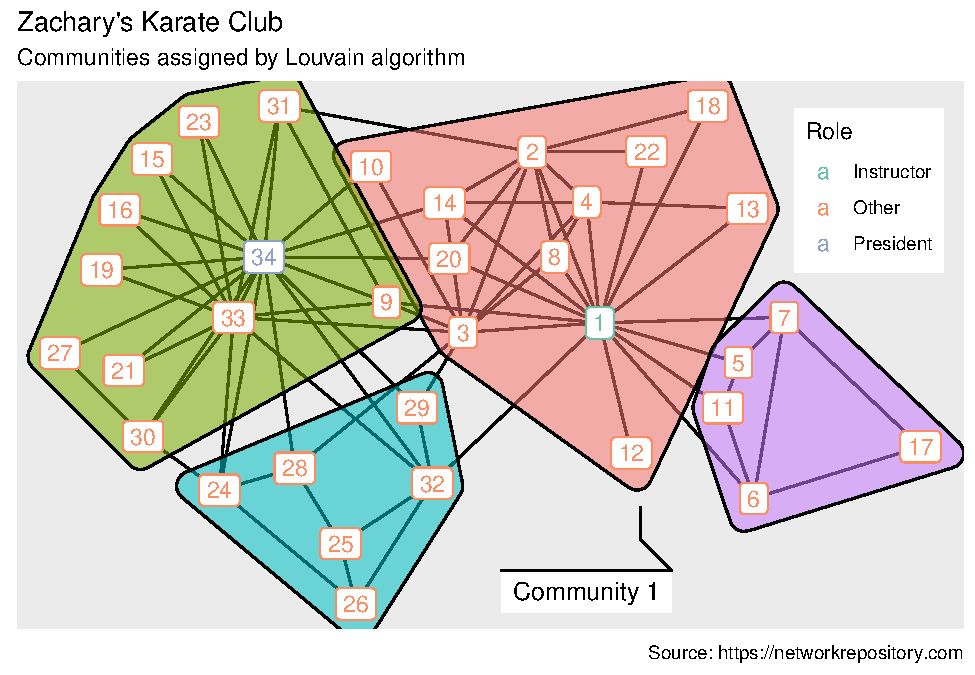
\includegraphics{Karate-Tasks_files/figure-latex/unnamed-chunk-12-1} \end{center}

\begin{enumerate}
\def\labelenumi{(\arabic{enumi})}
\setcounter{enumi}{11}
\tightlist
\item
  Briefly explain to a reader what the figure reveals about the
  karate-club network.
\end{enumerate}

\Ans From the figure, readers understand that there are 4 communities in
the karate-club network. Community 2 has the original president (of the
karate-club) and community 1 has the original instructor (community 1
has become his new organisation. From the black curve, we also know
where the observed split happened between the members of the
karate-club, the members that stayed in the old club were mainly from
community 2 and 3 (with the exception of 9 and 10).

\end{document}
